\documentclass[12pt]{beamer}
\usetheme{Frankfurt}
\usepackage[utf8]{inputenc}
\usepackage[english]{babel}
\usepackage{amsmath}
\usepackage{amsfonts}
\usepackage{amssymb}
\usepackage{booktabs}
% \author{Martin Dobiasch}
%\author{Martin \textsc{Dobiasch} \& Eugen \textsc{Havasi} \& Peter \textsc{Rjabcsenko}}
\author{Martin Dobiasch \& Eugen Havasi \& Peter Rjabcsenko}
%\title{}
%\setbeamercovered{transparent} 
%\setbeamertemplate{navigation symbols}{} 
%\logo{} 
%\institute{} 
%\date{} 
%\subject{} 
\begin{document}

\begin{frame}
\titlepage
\end{frame}

%\begin{frame}
%\tableofcontents
%\end{frame}

\begin{frame}{General Setup}
Python \& sklearn

\begin{block}{Algorithms}
\begin{itemize}
\item KNN
\item Decision Trees
\item Naive Bayes
\item SVM (SVR)
\end{itemize}
\end{block}

10 fold cross validation

Values reported are mean $\pm$ standard deviation

\end{frame}

\section{Communities}
\begin{frame}{Dataset}
Communities and Crime Data Set

Number of Instances: 1994

Number of Attributes: 128

Contains missing values

Task: Predict Violent Crimes per Population
\end{frame}

\begin{frame}{Initial view}
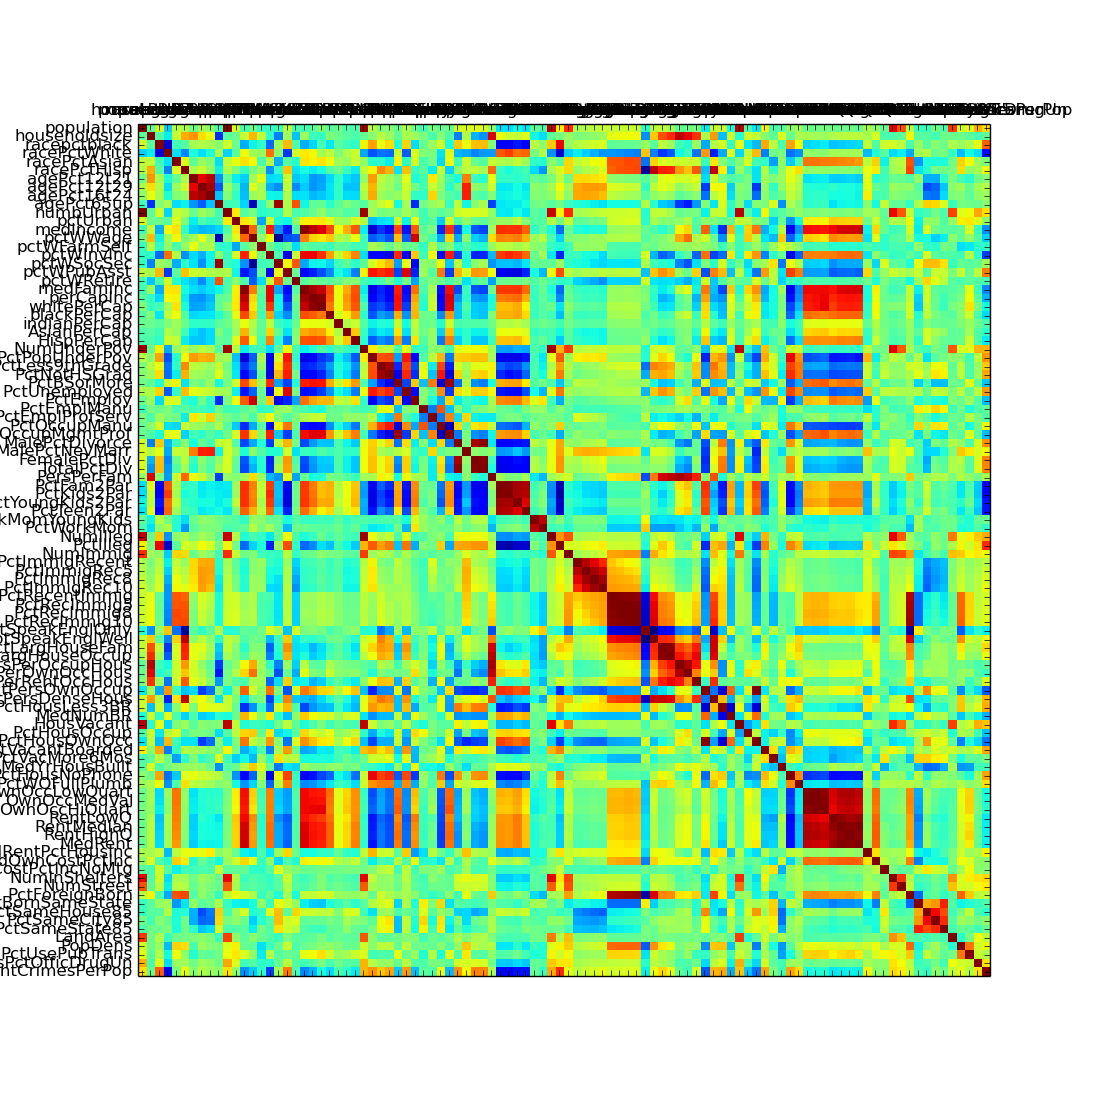
\includegraphics[height=\textheight,width=\textwidth,keepaspectratio]{plots/communities_orig.png}
\end{frame}

\begin{frame}{Preparations 1/2}
\begin{block}{Irrelevant}
state, county, community, communityname, fold

(from Dataset description)
\end{block}

\begin{block}{New Feature}
Recent Immigration: Split up 'recent', 'past 10', 'past 8', 'past 5' into '0 to 3', '3 to 5', '5 to 8', '8 to 10'
\end{block}
\end{frame}

\begin{frame}{Preparations 2/2}
\begin{block}{Side Notes}
''percentage of households with social security income in 1989''
correlates with ''percentage of population that is 65 and over in age''.

'percentage of people 16 and over who are employed in management or professional occupations'
correlates with ''percentage of people 25 and over with a bachelors degree or higher education''.
\end{block}

\begin{block}{After Cleaning}
Only 66 features left
\end{block}
\end{frame}

\begin{frame}{Final view}
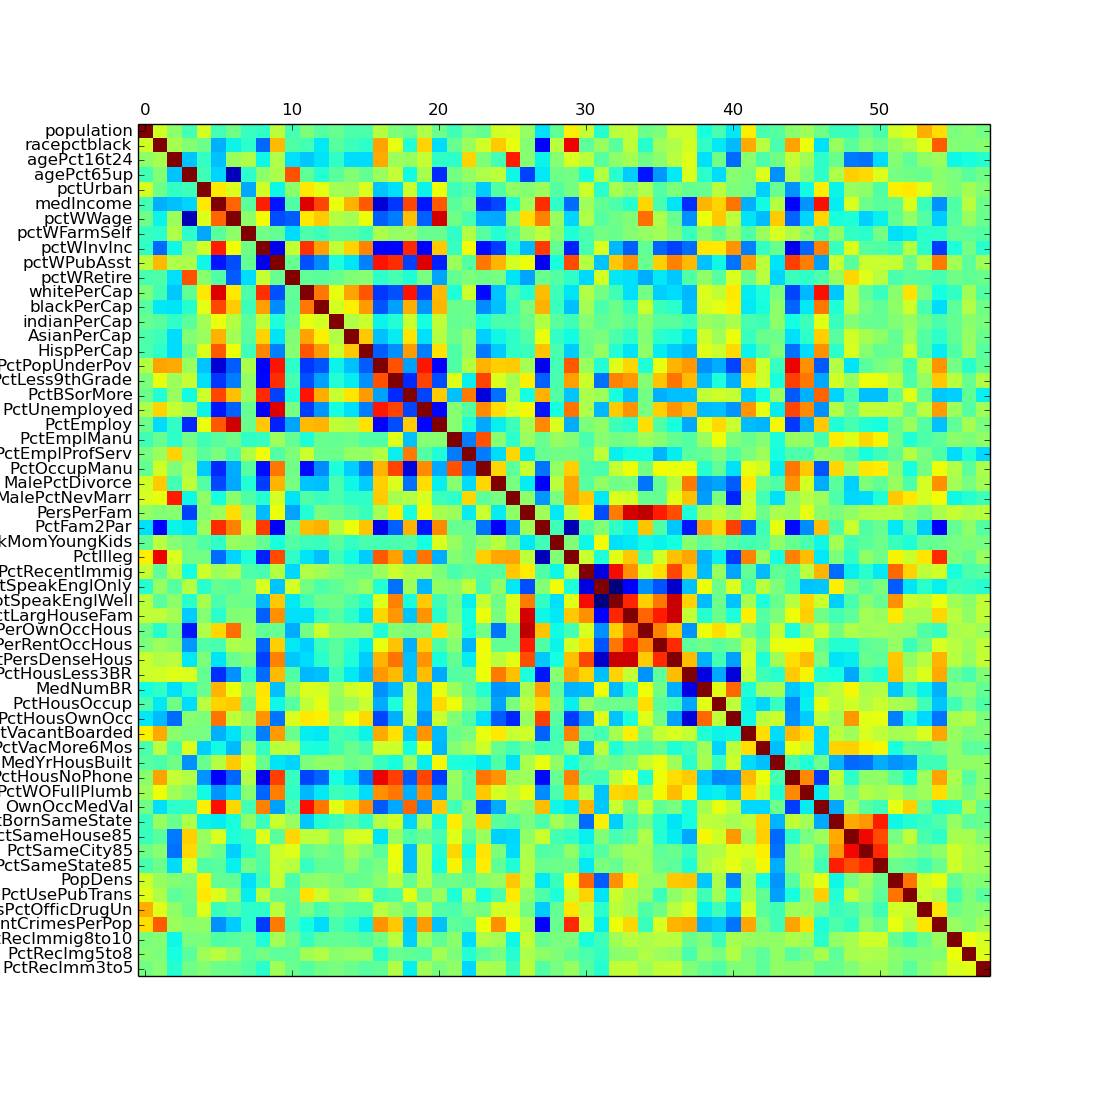
\includegraphics[height=\textheight,width=\textwidth,keepaspectratio]{plots/communities_final.png}
\end{frame}

\begin{frame}{Best parameters}
\begin{block}{KNN}
neighbors: 39, p: 1, weights: uniform
\end{block}

\begin{block}{Decision Tree}
'splitter': 'best', 'criterion': 'friedman\_mse', 'max\_features': 'auto'
\end{block}

\begin{block}{SVR}
'gamma': 0.1, 'C': 1, 'kernel': 'rbf'
\end{block}
\end{frame}

\begin{frame}{Results}
\resizebox{\linewidth}{!}{\begin{tabular}{lrrrrr}
\toprule
\textbf{Algorithm/Setting} & \textbf{time (ms)} & \textbf{time p (ms)} & \textbf{rmse} & \textbf{mae} & \textbf{cv}\\
\midrule
GaussianNB & $571.39 \pm 437.55$ & $27.67 \pm 13.26$ & $0.62 \pm 2.96$ & $0.44 \pm 2.08$ & $0.00 \pm 0.00$\\
\bottomrule
\end{tabular}
}
%KNN ({'n_neighbors': 39, 'p': 1, 'weights': 'uniform'}, 0.14411585292632384)
%Tree({'splitter': 'best', 'criterion': 'friedman_mse', 'max_features': 'auto'}, %0.14542545934079396)
%gnb ({}, 0.20893417278547977)
%svm ({'gamma': 0.1, 'C': 1, 'kernel': 'rbf'}, 0.20459216628575627)
\end{frame}

\section{Stock}
\begin{frame}{Dataset}
...

Number of Instances: 315

Number of Attributes: 12

No missing values

Task: ?

4 periods of data $\rightarrow$ accumulated data
\end{frame}

\begin{frame}{Initial/Final view}
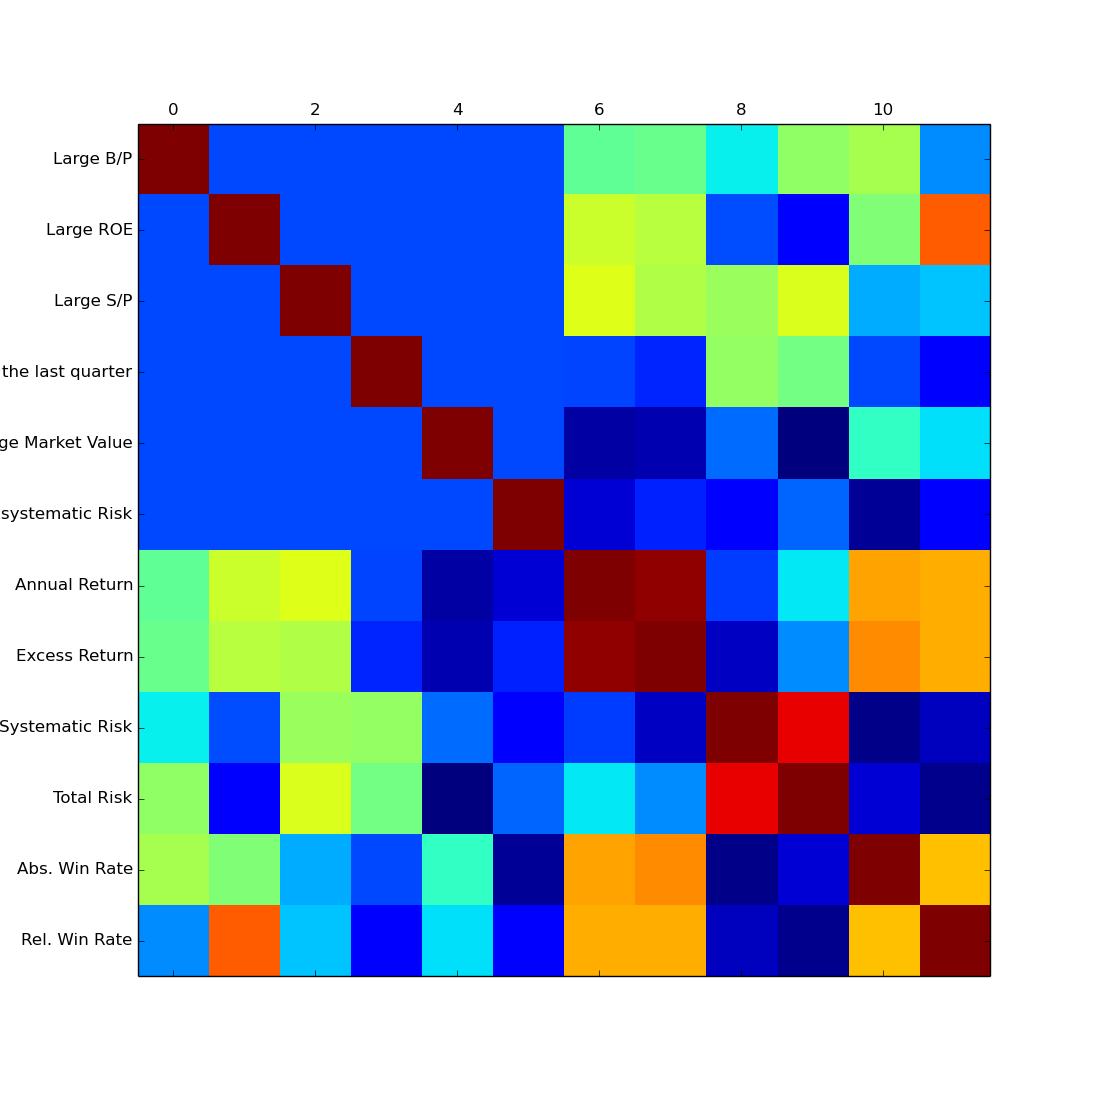
\includegraphics[height=\textheight,width=\textwidth,keepaspectratio]{plots/stock_final.png}
\end{frame}

\begin{frame}{Preprocessing}

\end{frame}

\begin{frame}{Results}
\resizebox{\linewidth}{!}{\begin{tabular}{lrrrrr}
\toprule
\textbf{Algorithm/Setting} & \textbf{time (ms)} & \textbf{time p (ms)} & \textbf{rmse} & \textbf{mae}\\
\midrule
SVR Rel. Win Rate & $3.31 \pm 22.30$ & $0.26 \pm 0.23$ & $38.24 \pm 915.69$ & $33.96 \pm 852.94$\\
GaussianNB Systematic Risk & $1.43 \pm 0.41$ & $0.29 \pm 0.25$ & $0.06 \pm 0.47$ & $0.05 \pm 0.40$\\
GaussianNB Total Risk & $4.63 \pm 28.96$ & $0.28 \pm 0.24$ & $64.24 \pm 1191.61$ & $57.08 \pm 1110.01$\\
GaussianNB Annual Return & $1.49 \pm 0.42$ & $0.45 \pm 0.24$ & $0.05 \pm 0.24$ & $0.04 \pm 0.19$\\
Decision Tree Systematic Risk & $1.42 \pm 0.39$ & $0.30 \pm 0.25$ & $0.03 \pm 0.12$ & $0.03 \pm 0.09$\\
GaussianNB Excess Return & $1.44 \pm 0.40$ & $0.32 \pm 0.25$ & $0.03 \pm 0.14$ & $0.03 \pm 0.11$\\
GaussianNB Rel. Win Rate & $3.45 \pm 23.08$ & $0.27 \pm 0.24$ & $40.64 \pm 948.01$ & $36.10 \pm 883.05$\\
Decision Tree Annual Return & $1.48 \pm 0.41$ & $0.56 \pm 0.17$ & $0.02 \pm 0.01$ & $0.01 \pm 0.01$\\
SVR Abs. Win Rate & $3.62 \pm 24.06$ & $0.26 \pm 0.23$ & $44.19 \pm 988.64$ & $39.26 \pm 920.90$\\
SVR Systematic Risk & $1.43 \pm 0.41$ & $0.29 \pm 0.25$ & $0.06 \pm 0.47$ & $0.05 \pm 0.40$\\
KNN Annual Return & $1.49 \pm 0.41$ & $0.57 \pm 0.16$ & $0.02 \pm 0.01$ & $0.01 \pm 0.01$\\
Decision Tree Rel. Win Rate & $3.45 \pm 23.09$ & $0.27 \pm 0.24$ & $40.68 \pm 948.52$ & $36.14 \pm 883.52$\\
KNN Systematic Risk & $1.41 \pm 0.39$ & $0.26 \pm 0.23$ & $0.02 \pm 0.12$ & $0.02 \pm 0.09$\\
SVR Annual Return & $1.41 \pm 0.39$ & $0.26 \pm 0.24$ & $0.04 \pm 0.16$ & $0.03 \pm 0.12$\\
Decision Tree Total Risk & $4.64 \pm 28.98$ & $0.28 \pm 0.24$ & $64.34 \pm 1192.62$ & $57.17 \pm 1110.95$\\
GaussianNB Abs. Win Rate & $3.91 \pm 25.52$ & $0.28 \pm 0.24$ & $49.78 \pm 1049.17$ & $44.23 \pm 977.29$\\
SVR Total Risk & $4.17 \pm 26.87$ & $0.26 \pm 0.23$ & $55.22 \pm 1105.06$ & $49.07 \pm 1029.36$\\
Decision Tree Abs. Win Rate & $3.91 \pm 25.54$ & $0.28 \pm 0.24$ & $49.84 \pm 1049.86$ & $44.28 \pm 977.94$\\
KNN Total Risk & $4.74 \pm 29.43$ & $0.29 \pm 0.24$ & $66.38 \pm 1211.29$ & $58.98 \pm 1128.34$\\
KNN Excess Return & $1.43 \pm 0.40$ & $0.33 \pm 0.25$ & $0.03 \pm 0.14$ & $0.02 \pm 0.11$\\
KNN Rel. Win Rate & $3.49 \pm 23.32$ & $0.28 \pm 0.24$ & $41.48 \pm 957.83$ & $36.85 \pm 892.20$\\
Decision Tree Excess Return & $1.44 \pm 0.40$ & $0.32 \pm 0.25$ & $0.03 \pm 0.13$ & $0.02 \pm 0.10$\\
SVR Excess Return & $1.41 \pm 0.39$ & $0.26 \pm 0.23$ & $0.02 \pm 0.12$ & $0.02 \pm 0.09$\\
KNN Abs. Win Rate & $3.97 \pm 25.85$ & $0.28 \pm 0.24$ & $51.05 \pm 1062.52$ & $45.36 \pm 989.73$\\
\bottomrule
\end{tabular}
}
%Annual Return
%({'p': 1, 'n_neighbors': 13, 'weights': 'distance'}, 0.017464444966712522)
%Best {'p': 1, 'n_neighbors': 13, 'weights': 'distance'}
%({'max_features': 'auto', 'splitter': 'best', 'criterion': 'friedman_mse'}, 0.017480511823369488)
%Best {'max_features': 'auto', 'splitter': 'best', 'criterion': 'friedman_mse'}
%({}, 0.045353596283597149)
%({'kernel': 'sigmoid', 'gamma': 100, 'C': 10000}, 0.037521455065540152)
%Best {'kernel': 'sigmoid', 'gamma': 100, 'C': 10000}
%Excess Return
%({'p': 2, 'n_neighbors': 14, 'weights': 'uniform'}, 0.029410711493046936)
%Best {'p': 2, 'n_neighbors': 14, 'weights': 'uniform'}
%({'max_features': 'sqrt', 'splitter': 'random', 'criterion': 'mse'}, 0.027639007161707793)
%Best {'max_features': 'sqrt', 'splitter': 'random', 'criterion': 'mse'}
%({}, 0.030747304462243566)
%({'kernel': 'sigmoid', 'gamma': 100, 'C': 10000}, 0.024376446796960709)
%Best {'kernel': 'sigmoid', 'gamma': 100, 'C': 10000}
%Systematic Risk
%({'p': 1, 'n_neighbors': 1, 'weights': 'distance'}, 0.024608917252478796)
%Best {'p': 1, 'n_neighbors': 1, 'weights': 'distance'}
%({'max_features': 'auto', 'splitter': 'best', 'criterion': 'friedman_mse'}, 0.031696405813183427)
%Best {'max_features': 'auto', 'splitter': 'best', 'criterion': 'friedman_mse'}
%({}, 0.05533186206973556)
%({'kernel': 'linear', 'gamma': 0.001, 'C': 10}, 0.055430927962504581)
%Best {'kernel': 'linear', 'gamma': 0.001, 'C': 10}
%Total Risk
%({'p': 2, 'n_neighbors': 14, 'weights': 'uniform'}, 66.379581864771779)
%Best {'p': 2, 'n_neighbors': 14, 'weights': 'uniform'}
%({'max_features': 'sqrt', 'splitter': 'random', 'criterion': 'mse'}, 64.344454982589511)
%Best {'max_features': 'sqrt', 'splitter': 'random', 'criterion': 'mse'}
%({}, 64.237512184944563)
%({'kernel': 'sigmoid', 'gamma': 100, 'C': 10000}, 55.224220447355592)
%Best {'kernel': 'sigmoid', 'gamma': 100, 'C': 10000}
%Abs. Win Rate
%({'p': 2, 'n_neighbors': 14, 'weights': 'uniform'}, 51.047246411047887)
%Best {'p': 2, 'n_neighbors': 14, 'weights': 'uniform'}
%({'max_features': 'sqrt', 'splitter': 'random', 'criterion': 'mse'}, 49.83591746228614)
%Best {'max_features': 'sqrt', 'splitter': 'random', 'criterion': 'mse'}
%({}, 49.776696369867437)
%({'kernel': 'sigmoid', 'gamma': 100, 'C': 10000}, 44.192224269048054)
%Best {'kernel': 'sigmoid', 'gamma': 100, 'C': 10000}
%Rel. Win Rate
%({'p': 2, 'n_neighbors': 14, 'weights': 'uniform'}, 41.478207993268704)
%Best {'p': 2, 'n_neighbors': 14, 'weights': 'uniform'}
%({'max_features': 'sqrt', 'splitter': 'random', 'criterion': 'mse'}, 40.675461749113211)
%Best {'max_features': 'sqrt', 'splitter': 'random', 'criterion': 'mse'}
%({}, 40.6361006383042)
%({'kernel': 'rbf', 'gamma': 10, 'C': 1000}, 38.240834600476589)
%Best {'kernel': 'rbf', 'gamma': 10, 'C': 1000}

\end{frame}


\section{Auto}
\begin{frame}{Initial/Final view}
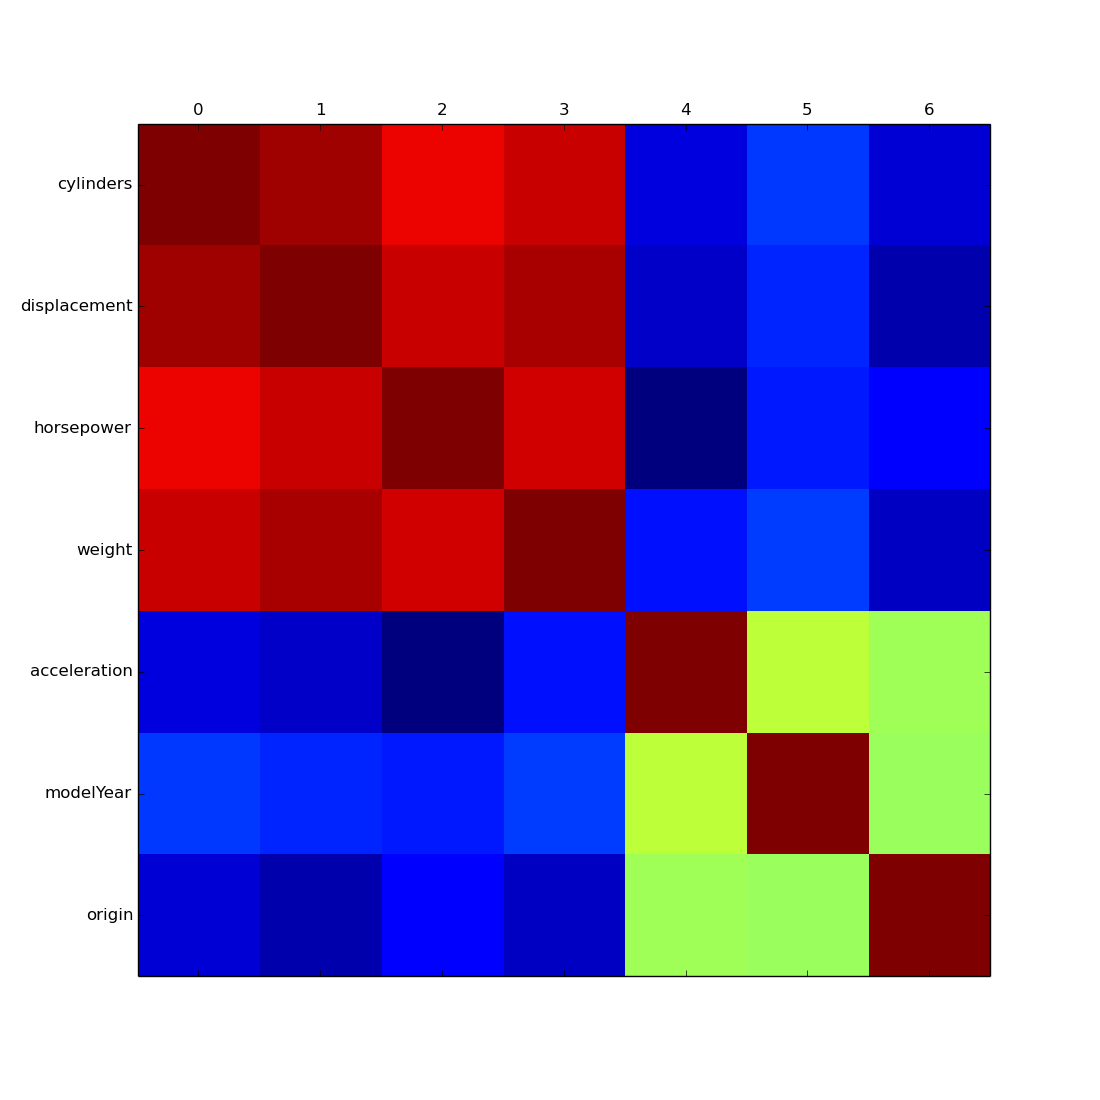
\includegraphics[height=\textheight,width=\textwidth,keepaspectratio]{plots/auto_final.png}
\end{frame}

\begin{frame}{Preprocessing}

\end{frame}

\begin{frame}{Best Parameters}
%({'weights': 'uniform', 'n_neighbors': 291, 'p': 2}, 4.1350573536016384)
%Best {'weights': 'uniform', 'n_neighbors': 291, 'p': 2}
%({'splitter': 'best', 'max_features': 'auto', 'criterion': 'friedman_mse'}, 4.1554836861671154)
%Best {'splitter': 'best', 'max_features': 'auto', 'criterion': 'friedman_mse'}
%({}, 4.4882746764655668)
\begin{block}{KNN}
neighbors: 291, p: 2, weights: uniform
\end{block}

\begin{block}{Decision Tree}
'splitter': 'best', 'criterion': 'friedman\_mse', 'max\_features': 'auto'
\end{block}

\begin{block}{SVR}

\end{block}
\end{frame}

\begin{frame}{Results}
%\resizebox{\linewidth}{!}{\begin{tabular}{lrrrrr}
\toprule
\textbf{Algorithm/Setting} & \textbf{time (ms)} & \textbf{time p (ms)} & \textbf{rmse} & \textbf{mae} & \textbf{cv}\\
\midrule
Decision Tree & $4.33 \pm 1.75$ & $0.95 \pm 0.39$ & $33.04 \pm 9.00$ & $24.89 \pm 6.88$ & $nan \pm nan$\\
KNN & $4.58 \pm 1.59$ & $0.95 \pm 0.36$ & $31.18 \pm 8.11$ & $23.27 \pm 5.89$ & $nan \pm nan$\\
SVR & $4.74 \pm 2.44$ & $0.90 \pm 0.70$ & $34.09 \pm 9.99$ & $25.63 \pm 7.74$ & $nan \pm nan$\\
GaussianNB & $4.74 \pm 2.44$ & $0.91 \pm 0.70$ & $33.77 \pm 9.24$ & $25.33 \pm 6.86$ & $nan \pm nan$\\
\bottomrule
\end{tabular}
}
\end{frame}

\section{KDD}
\begin{frame}{Initial view}
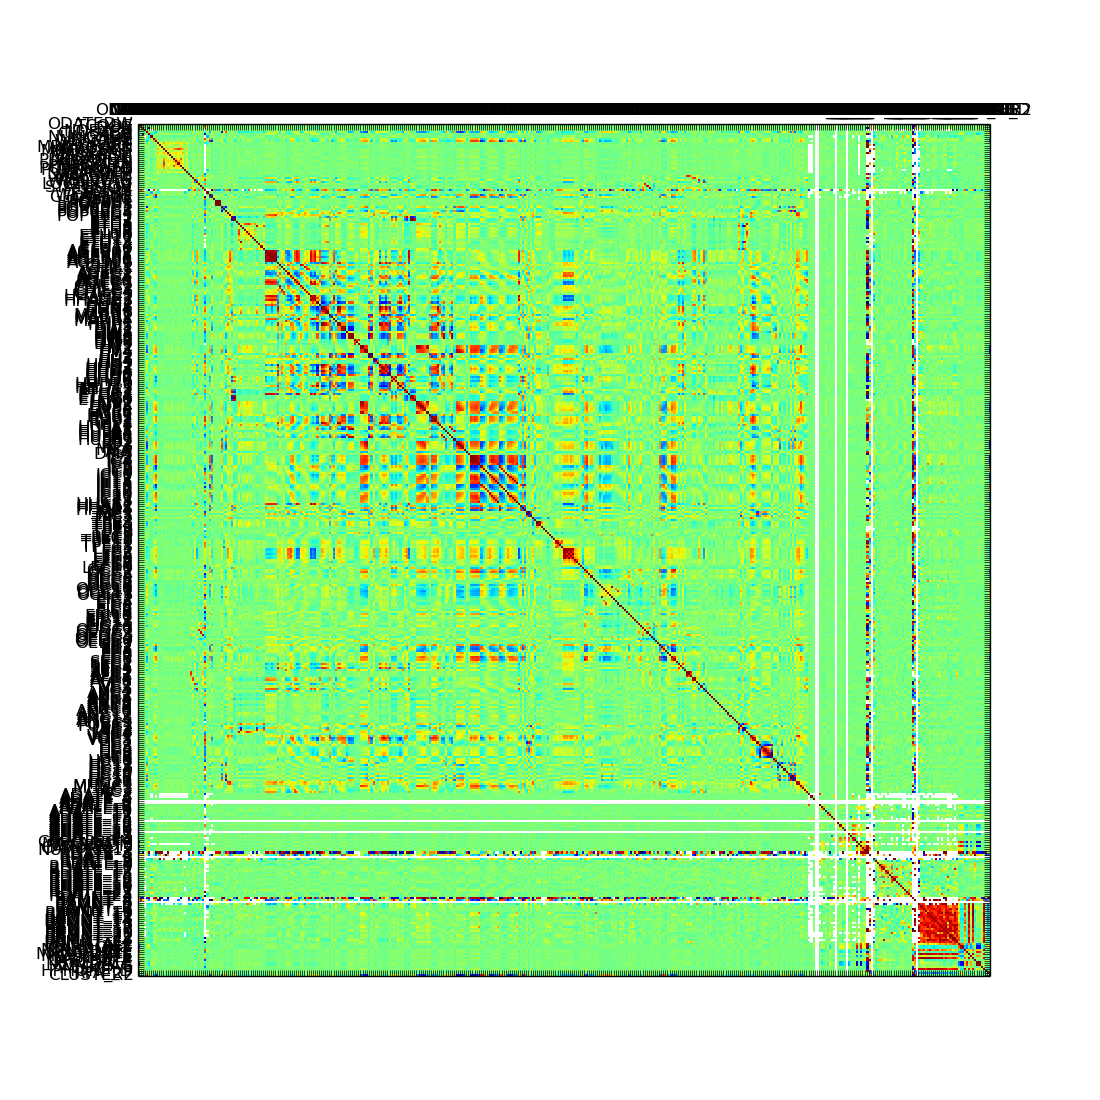
\includegraphics[height=\textheight,width=\textwidth,keepaspectratio]{plots/kdd_orig.png}
\end{frame}

\begin{frame}{Preprocessing}

\end{frame}

\begin{frame}{Final view}
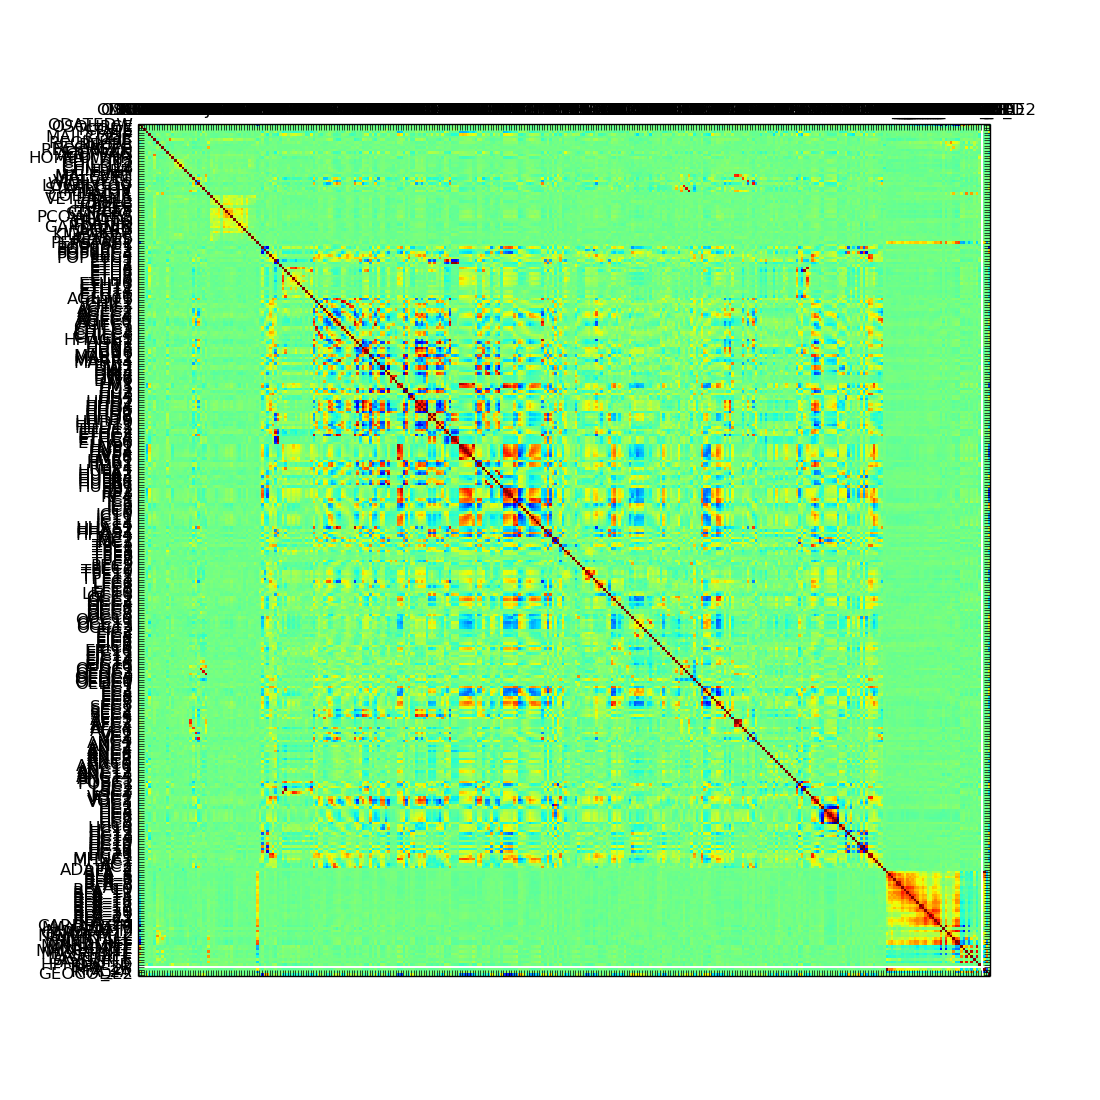
\includegraphics[height=\textheight,width=\textwidth,keepaspectratio]{plots/kdd_final.png}
\end{frame}

\begin{frame}{Findings}
Imputing mean vs. removing cols with missing values: latter gives better results

\begin{block}{KNN}
neighbors: 291, p: 2, weights: uniform
\end{block}

\begin{block}{Decision Tree}
'splitter': 'best', 'criterion': 'friedman\_mse', 'max\_features': 'auto'
\end{block}

\begin{block}{SVR}

\end{block}
% results from removing:
% ({'n_neighbors': 291, 'p': 2, 'weights': 'uniform'}, 4.1350573536016384)
% ({'splitter': 'best', 'criterion': 'friedman_mse', 'max_features': 'auto'}, 4.1544598320715354)
% Results from imputing mean
% ({'n_neighbors': 291, 'p': 2, 'weights': 'uniform'}, 4.289451889295445)
% ({'splitter': 'best', 'criterion': 'friedman_mse', 'max_features': 'auto'}, 4.2979202497555358)
\end{frame}

\begin{frame}{Results}
\resizebox{\linewidth}{!}{\begin{tabular}{lrrrrr}
\toprule
\textbf{Algorithm/Setting} & \textbf{time (ms)} & \textbf{time p (ms)} & \textbf{rmse} & \textbf{mae}\\
\midrule
KNN IM & $3883.10 \pm 21788.33$ & $443.38 \pm 323.80$ & $6.97 \pm 53.39$ & $2.09 \pm 9.84$\\
GaussianNB RM & $353.68 \pm 2524.32$ & $513.90 \pm 235.96$ & $4.49 \pm 1.36$ & $1.70 \pm 0.83$\\
SVR IM & $3652.78 \pm 19154.44$ & $370.17 \pm 336.05$ & $6.44 \pm 46.61$ & $1.93 \pm 8.61$\\
SVR RM & $937.16 \pm 2609.10$ & $365.49 \pm 283.08$ & $4.41 \pm 1.22$ & $1.52 \pm 0.87$\\
KNN RM & $36.35 \pm 7.79$ & $595.17 \pm 127.21$ & $4.14 \pm 0.84$ & $1.60 \pm 0.14$\\
GaussianNB IM & $3827.58 \pm 21349.76$ & $423.45 \pm 329.47$ & $6.96 \pm 52.17$ & $2.10 \pm 9.62$\\
Decision Tree IM & $3836.62 \pm 21374.29$ & $424.44 \pm 329.23$ & $6.95 \pm 52.23$ & $2.08 \pm 9.63$\\
Decision Tree RM & $42.90 \pm 73.42$ & $590.25 \pm 137.65$ & $4.16 \pm 0.87$ & $1.60 \pm 0.14$\\
\bottomrule
\end{tabular}
}
\end{frame}

\section{Summary}
\begin{frame}
\begin{block}{Runtimes}
Used different PCs for testing $\rightarrow$ no real runtime measurements
\end{block}

Search space too large

More imputation strategies?

No feature selection

No autosklearn
\end{frame}

\end{document}